\section*{Resumen}
En este informe se presenta el diseño, construcción y validación experimental de un prototipo casero de excavadora hidráulica articulada de cuatro grados de libertad, desarrollado como trabajo práctico de la unidad de aprendizaje de Física en la Facultad de Agronomía de la Universidad Autónoma de Nuevo León. El mecanismo fundamenta su funcionamiento en el Principio de Pascal y en la transmisión hidrostática de presión en fluidos incompresibles. A partir del diagrama de piezas prefabricadas en madera de \SI{3}{mm}, se integraron ocho cilindros hipodérmicos interconectados en parejas mediante mangueras flexibles y una consola manual de mando. Como fluido de transmisión se empleó agua desgasificada con trazador fucsia para asegurar la eliminación absoluta de burbujas de aire. Las pruebas cinemáticas sobre sustrato de cultivo validaron la ventaja mecánica del sistema, alcanzando un barrido angular de \SI{170}{\degree} y levantando cargas de suelo de hasta \SI{120}{g}, demostrando empíricamente los principios hidrostáticos aplicados en la maquinaria pesada de zanjado y drenaje parcelario.

\vspace{0.3cm}
\noindent\textbf{Palabras clave:} Principio de Pascal, transmisión hidráulica, excavadora articulada, mecánica de fluidos, maquinaria agrícola, incompresibilidad.

\clearpage

\section{Introducción y Fundamento Físico de la Hidráulica}

\subsection{Justificación Agronómica de la Hidráulica Móvil}
En la actividad agrícola contemporánea, la maquinaria pesada para movimiento de tierras ---como retroexcavadoras, zanjadoras y palas mecánicas--- resulta indispensable para la infraestructura productiva \parencite{ortiz2003}. Estas máquinas ejecutan labores críticas tales como el trazado de canales de drenaje parcelario para evitar la salinización de los horizontes superficiales, la excavación de zanjas para el enterramiento de líneas presurizadas de riego por goteo, la remoción de horizontes compactados o tepetate, y el despalme de terrenos para invernaderos.

El principio operativo que gobierna la totalidad de los actuadores en estas máquinas es la oleohidráulica. Para un estudiante de Ingeniería Agronómica, el dominio conceptual y empírico de la mecánica de fluidos constituye una base indispensable para entender la transmisión de esfuerzos masivos con bajo consumo de potencia, la operación de cilindros de simple y doble efecto, y los requerimientos de mantenimiento y purga de circuitos presurizados.

\subsection{Principio de Pascal y Leyes Hidrostáticas}
El comportamiento de los circuitos de transmisión de potencia fluídica se rige por la ley enunciada por el físico francés Blaise Pascal en 1653: \textit{la presión ejercida sobre un fluido incompresible y en equilibrio dentro de un recipiente de paredes indeformables se transmite con idéntica intensidad en todas las direcciones y en todos los puntos del fluido} \parencite{tippens2011,perezmontiel2014}.

La presión hidrostática $P$ originada por una fuerza perpendicular $F_1$ aplicada sobre un émbolo de sección transversal $A_1$ se define como:
\begin{equation}
    P = \frac{F_1}{A_1}
    \label{eq:presion_pascal}
\end{equation}

Al encontrarse este cilindro emisor conectado mediante un conducto cerrado y flexible a un cilindro receptor de área $A_2$, la presión generada se propaga íntegramente hacia el segundo pistón ($P_1 = P_2$). Por consiguiente, la fuerza de salida $F_2$ desarrollada por el cilindro receptor resulta:
\begin{equation}
    \frac{F_1}{A_1} = \frac{F_2}{A_2} \implies F_2 = F_1 \left( \frac{A_2}{A_1} \right)
    \label{eq:fuerza_multiplicada}
\end{equation}

Esta expresión matemática establece la \textbf{ventaja mecánica hidráulica} del sistema:
\begin{itemize}
    \item Si el área del émbolo receptor $A_2$ es superior al área del émbolo emisor $A_1$, la fuerza de salida se magnifica en proporción al cociente de áreas:
    \begin{equation}
        \text{VM} = \frac{A_2}{A_1} = \left(\frac{d_2}{d_1}\right)^2
    \end{equation}
    \item Si ambas jeringas poseen idéntico diámetro ($A_1 = A_2$), el sistema opera como un transmisor de desplazamiento directo con ganancia unitaria, garantizando un control posicional preciso e instantáneo.
\end{itemize}

Asimismo, considerando que los líquidos presentan una compresibilidad casi nula a presiones de trabajo ordinarias, el volumen desplazado por el pistón emisor ($V_1 = A_1 \cdot \Delta x_1$) debe ser estrictamente igual al volumen admitido por el pistón receptor ($V_2 = A_2 \cdot \Delta x_2$):
\begin{equation}
    A_1 \cdot \Delta x_1 = A_2 \cdot \Delta x_2 \implies \Delta x_2 = \Delta x_1 \left( \frac{A_1}{A_2} \right)
    \label{eq:desplazamiento}
\end{equation}

De esta manera, el principio de conservación de la energía mecánica se cumple puntualmente: la multiplicación de fuerza obtenida en el actuador se compensa con una reducción proporcional en la carrera lineal del vástago.


\section{Componentes, Dimensionamiento y Esquema General}

\subsection{Esquema General del Modelo y Distribución de Piezas}
El mecanismo reproduce a escala el tren cinemático de una excavadora pesada sobre chasis fijo de madera. En la Figura \ref{fig:diagramas_kit} se presentan el inventario estructurado de componentes del kit y la perspectiva general del modelo ensamblado, indicando la ubicación relativa de las jeringas de mando y los cilindros actuadores.

\begin{figure}[!htb]
    \centering
    \begin{subfigure}[b]{0.48\textwidth}
        \centering
        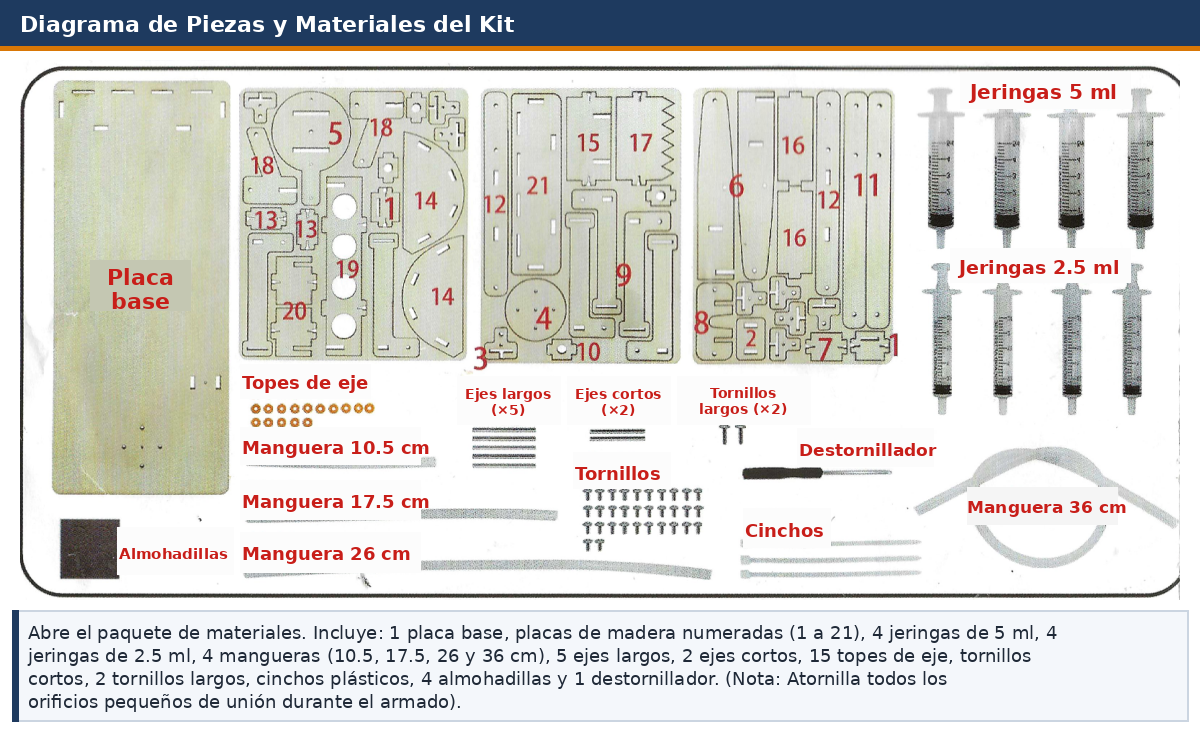
\includegraphics[width=\textwidth,height=4.8cm,keepaspectratio]{UANL/ingeniero-agronomo/fisica/figuras-pia/kit_piezas_materiales.png}
        \caption{Diagrama de piezas de madera numeradas y materiales del kit.}
        \label{fig:piezas_kit}
    \end{subfigure}
    \hfill
    \begin{subfigure}[b]{0.48\textwidth}
        \centering
        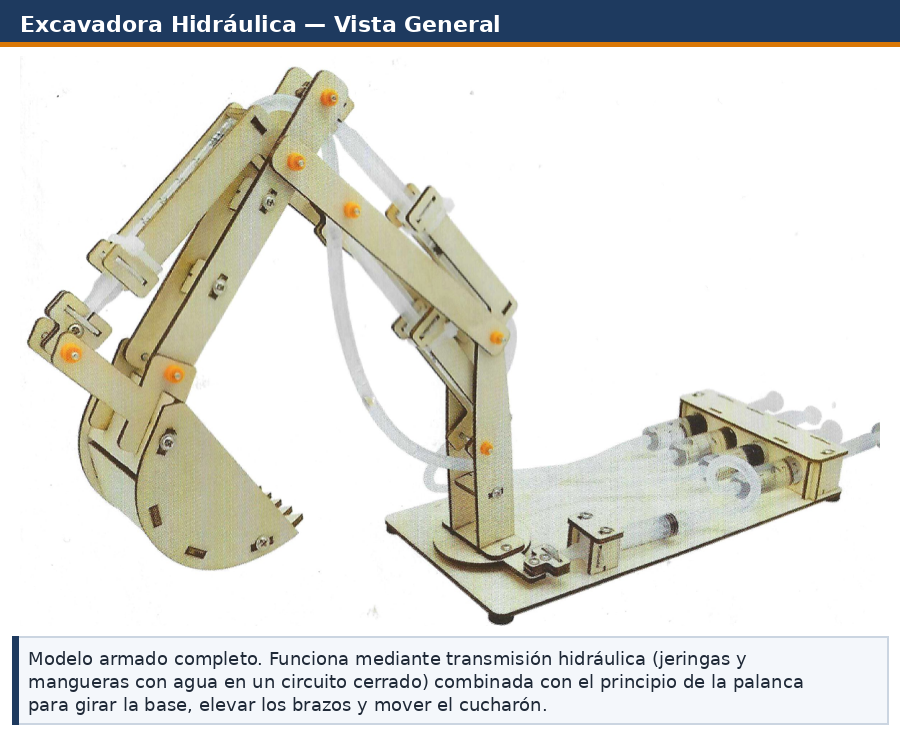
\includegraphics[width=\textwidth,height=4.8cm,keepaspectratio]{UANL/ingeniero-agronomo/fisica/figuras-pia/modelo_vista_general.png}
        \caption{Excavadora hidráulica montada: vista general del mecanismo.}
        \label{fig:modelo_general}
    \end{subfigure}
    \caption{Componentes de ingeniería del manipulador: despiece dimensional de placas de madera contrachapada y ensamble general de los cuatro ejes.}
    \label{fig:diagramas_kit}
\end{figure}

\subsection{Distribución Cinemática de los Cuatro Grados de Libertad}
El manipulador opera mediante cuatro movimientos articulares desacoplados:
\begin{enumerate}
    \item \textbf{Eje 1 (Giro Azimutal de la Base):} Articulación pivotante gobernada por el Cilindro 0 alojado sobre la placa base, con capacidad de rotación horizontal de hasta \SI{170}{\degree} para vaciado lateral.
    \item \textbf{Eje 2 (Elevación de la Pluma):} Cilindro 1 fijado en la base del soporte vertical que vence el mayor momento flector contra la gravedad para elevar el brazo completo.
    \item \textbf{Eje 3 (Extensión del Brazo / Pilar):} Cilindro 2 montado sobre el lomo de la pluma que aproxima o aleja la herramienta de excavación.
    \item \textbf{Eje 4 (Vuelco del Cucharón Zanjador):} Cilindro 3 vinculado a la cuchara dentada para efectuar el desgarre, carga y descarga de terrones.
\end{enumerate}


\section{Proceso de Construcción y Montaje Metodológico}

\subsection{Secuencia de Ensamble Mecánico y Circuitos Hidráulicos}
Dado que las fichas de construcción integran sus propias especificaciones de piezas y notas operativas, en la Figura \ref{fig:secuencia_construccion} se sintetizan visualmente las etapas clave del ensamble organizadas cronológicamente en tres líneas de proceso.

\begin{figure}[!htb]
    \centering
    % Renglón 1: Base giratoria y actuadores
    \begin{subfigure}[b]{0.48\textwidth}
        \centering
        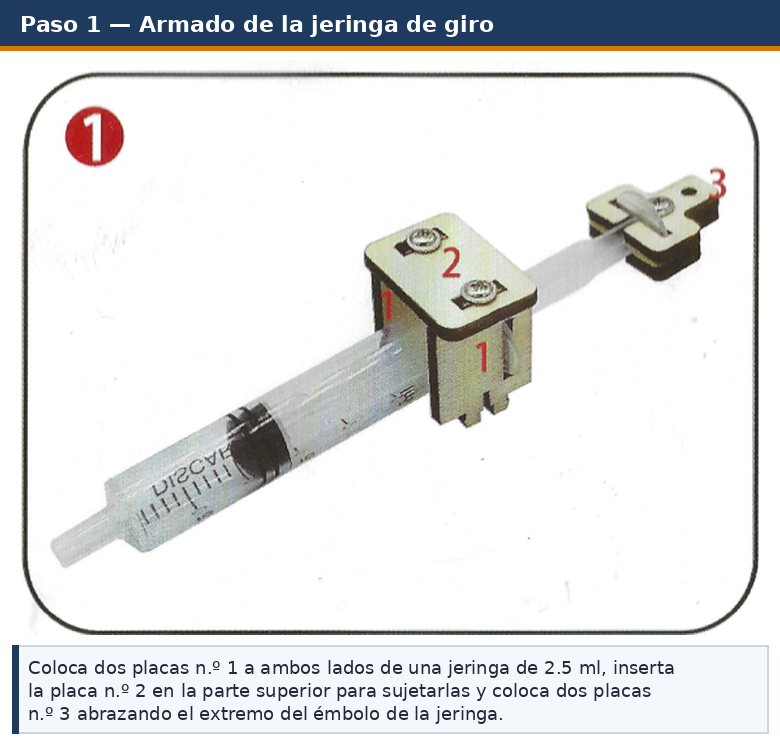
\includegraphics[width=\textwidth,height=3.9cm,keepaspectratio]{UANL/ingeniero-agronomo/fisica/figuras-pia/paso_01_armado_giro.png}
        \caption{Paso 1: Jeringa y soporte de giro azimutal.}
        \label{fig:paso1}
    \end{subfigure}
    \hfill
    \begin{subfigure}[b]{0.48\textwidth}
        \centering
        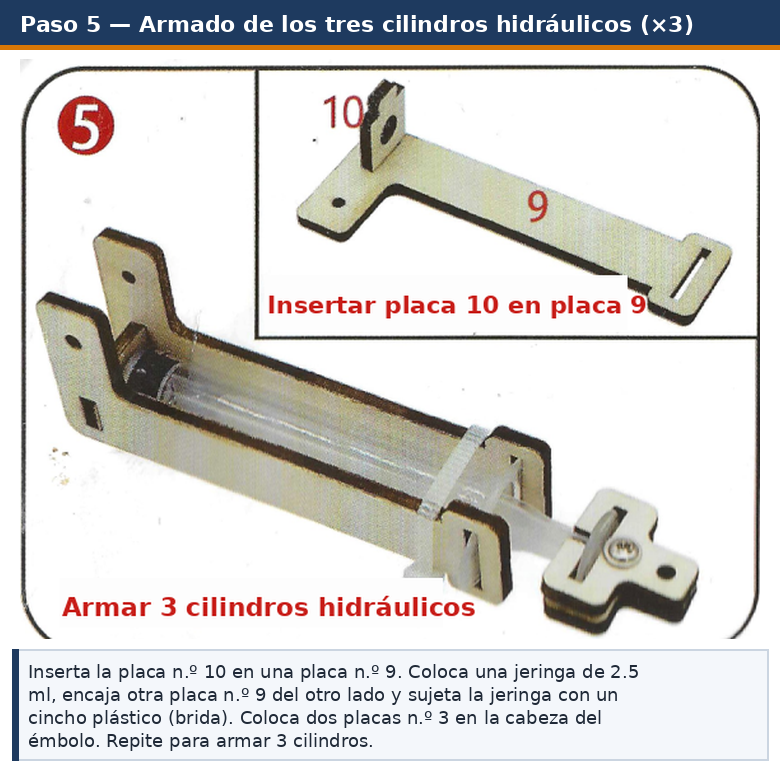
\includegraphics[width=\textwidth,height=3.9cm,keepaspectratio]{UANL/ingeniero-agronomo/fisica/figuras-pia/paso_05_tres_cilindros.png}
        \caption{Paso 5: Armado de los tres cilindros hidráulicos.}
        \label{fig:paso5}
    \end{subfigure}
    \vspace{0.20cm}

    % Renglón 2: Articulación mecánica de brazos y cucharón
    \begin{subfigure}[b]{0.48\textwidth}
        \centering
        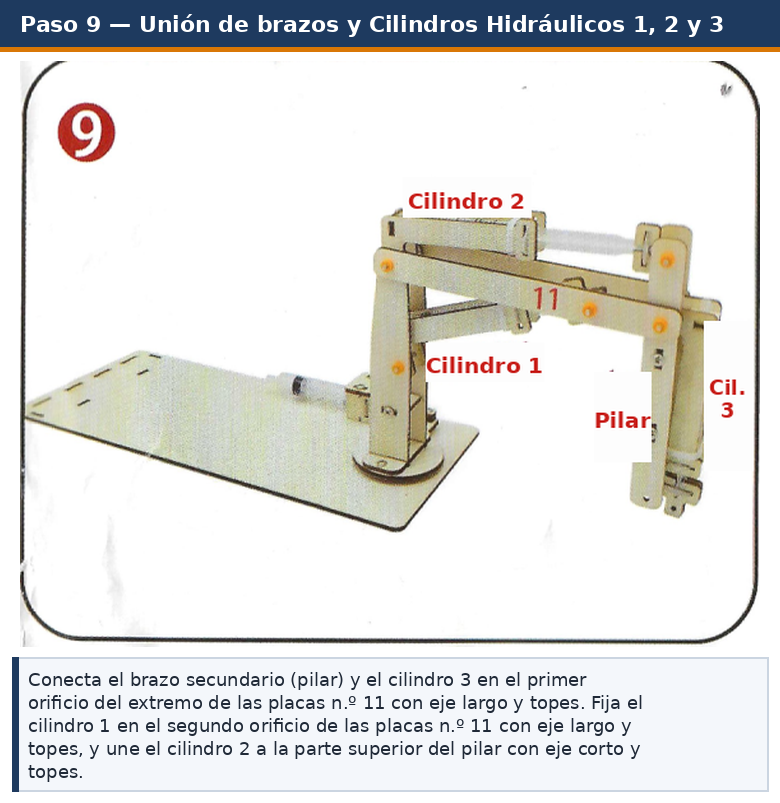
\includegraphics[width=\textwidth,height=3.9cm,keepaspectratio]{UANL/ingeniero-agronomo/fisica/figuras-pia/paso_09_union_brazos.png}
        \caption{Paso 9: Articulación de pluma, brazo y cilindros.}
        \label{fig:paso9}
    \end{subfigure}
    \hfill
    \begin{subfigure}[b]{0.48\textwidth}
        \centering
        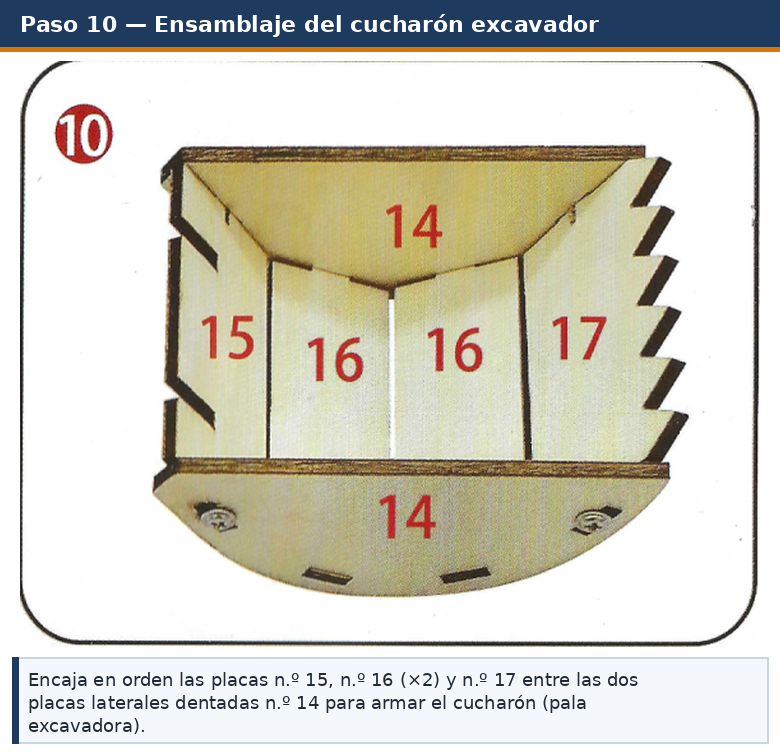
\includegraphics[width=\textwidth,height=3.9cm,keepaspectratio]{UANL/ingeniero-agronomo/fisica/figuras-pia/paso_10_cucharon.png}
        \caption{Paso 10: Ensamblaje del cucharón zanjador.}
        \label{fig:paso10}
    \end{subfigure}
    \vspace{0.20cm}

    % Renglón 3: Conexionado de mangueras y consola de control
    \begin{subfigure}[b]{0.48\textwidth}
        \centering
        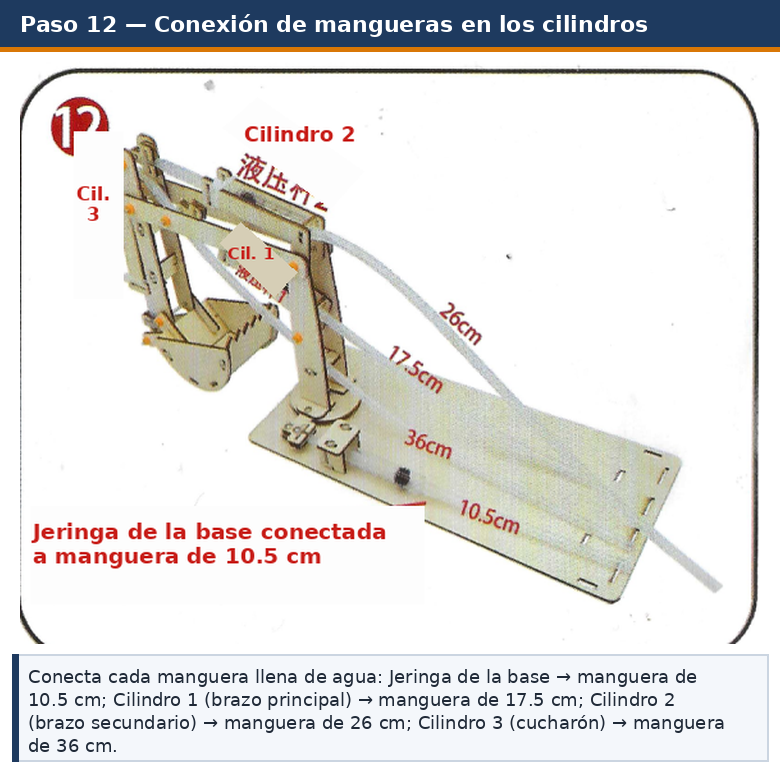
\includegraphics[width=\textwidth,height=3.9cm,keepaspectratio]{UANL/ingeniero-agronomo/fisica/figuras-pia/paso_12_mangueras.png}
        \caption{Paso 12: Tendido de mangueras hidráulicas.}
        \label{fig:paso12}
    \end{subfigure}
    \hfill
    \begin{subfigure}[b]{0.48\textwidth}
        \centering
        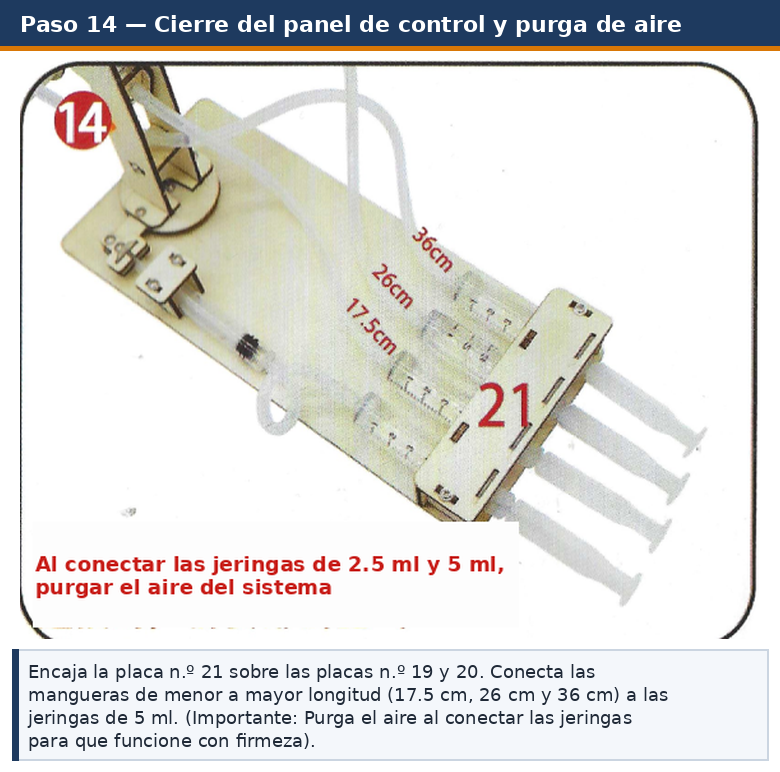
\includegraphics[width=\textwidth,height=3.9cm,keepaspectratio]{UANL/ingeniero-agronomo/fisica/figuras-pia/paso_14_panel_purga.png}
        \caption{Paso 14: Consola de control y purga de aire.}
        \label{fig:paso14}
    \end{subfigure}
    \caption{Secuencia metodológica de construcción (dos fases por renglón): subensambles mecánicos, conexionado hidráulico acotado y purga final de la consola.}
    \label{fig:secuencia_construccion}
\end{figure}

\subsection{Purga Hidrostática y Confiabilidad Operativa}
La desgasificación del fluido constituyó la fase más crítica del montaje. Se sumergieron las jeringas y los conductos de vinilo en un recipiente hondo con agua coloreada, acoplando los terminales bajo agua para expulsar el \SI{100}{\%} del aire atrapado. Las boquillas se aseguraron con cinta teflón y bridas de nylon para resistir las presiones de empuje sin deslizamientos ni fugas.


\subsection{Prototipo Físico Tangible Terminado}
En la Figura \ref{fig:foto_real_terminada} se aprecia la fotografía real del prototipo físico manufacturado, donde se constatan la adecuada tensión de las mangueras flexibles, el líquido fucsia uniforme en todos los actuadores y la robustez de los pernos de sujeción.

\begin{figure}[!htb]
    \centering
    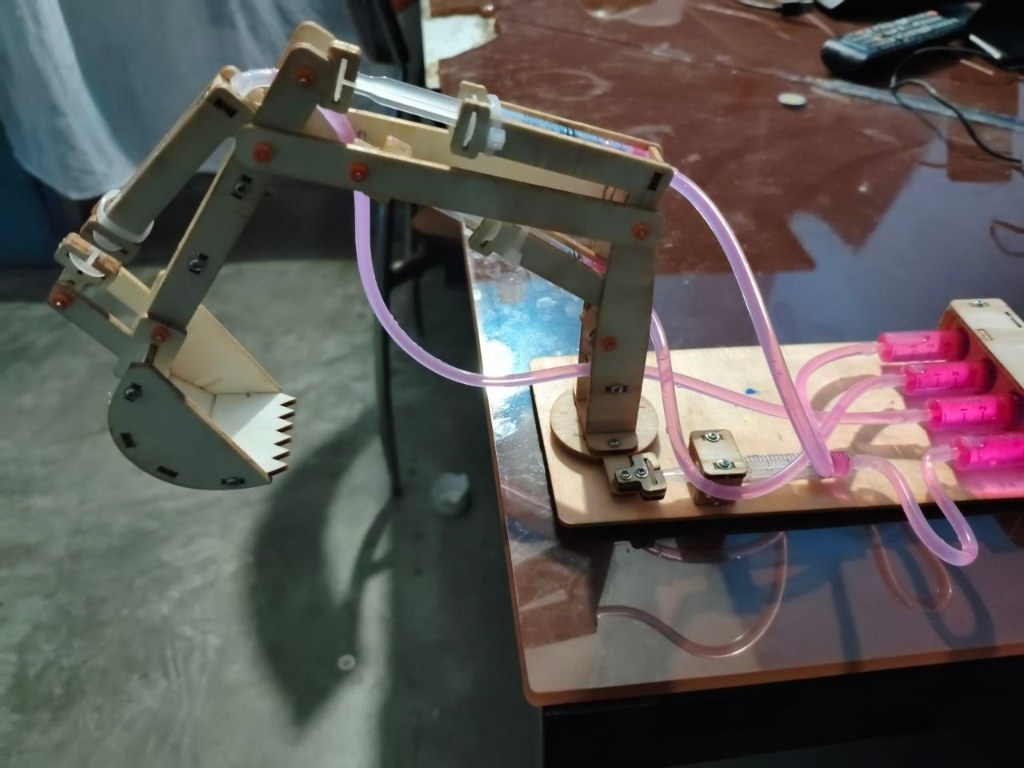
\includegraphics[width=0.82\textwidth,height=4.2cm,keepaspectratio]{UANL/ingeniero-agronomo/fisica/figuras-pia/foto_real_lateral.jpg}
    \caption{Prototipo físico terminado y operativo: vista lateral completa mostrando la consola de mando de cuatro vías, el tendido hidráulico con fluido teñido y la cuchara zanjadora dentada montada.}
    \label{fig:foto_real_terminada}
\end{figure}

\section{Ensayos Experimentales, Cinemática y Resultados}

\subsection{Pruebas de Operación en Sustrato Agrícola}
Para evaluar la respuesta cinemática y la resistencia estructural, se sometió el prototipo a ciclos de trabajo continuo sobre una charola con tierra vegetal húmeda de cultivo (humedad gravimétrica aproximada del \SI{22}{\%}).

Se midieron experimentalmente las carreras lineales de cada cilindro, los ángulos barridos en cada articulación y la capacidad de carga efectiva de la cuchara zanjadora (Figura \ref{fig:foto_cenital_operacion}).

\begin{figure}[!htb]
    \centering
    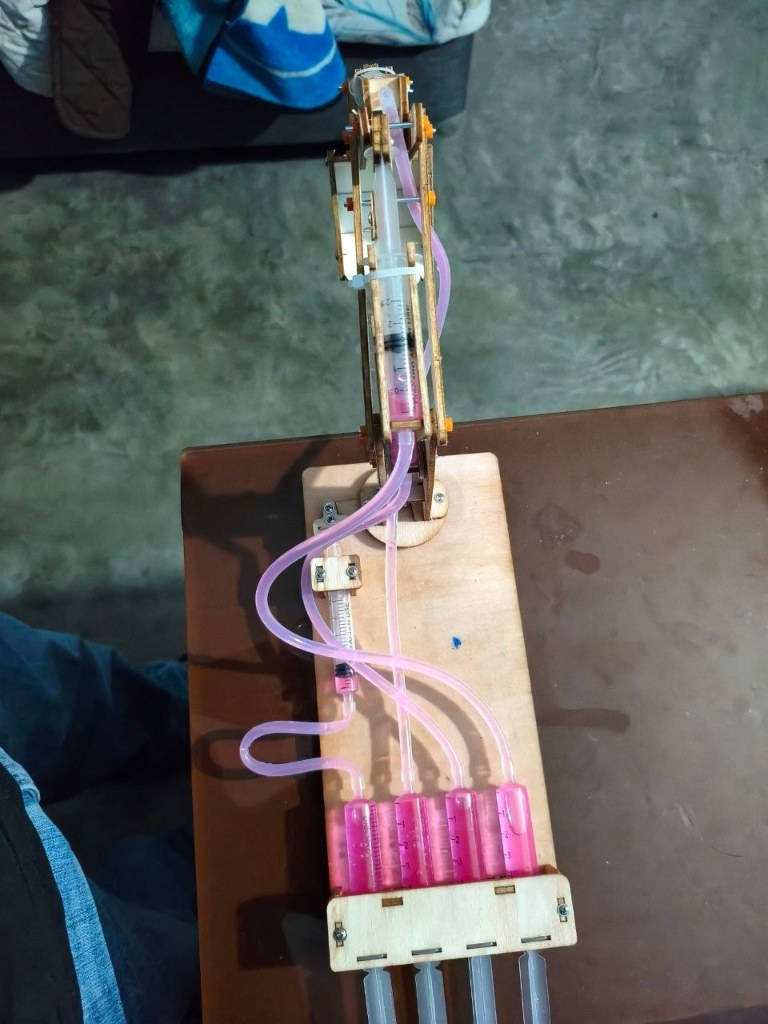
\includegraphics[width=0.72\textwidth,height=4.2cm,keepaspectratio]{UANL/ingeniero-agronomo/fisica/figuras-pia/foto_real_superior.jpg}
    \caption{Vista cenital del prototipo durante los ensayos de operación continua, mostrando el radio de alcance y barrido angular de la excavadora.}
    \label{fig:foto_cenital_operacion}
\end{figure}

Los resultados cuantitativos obtenidos en las mediciones cinemáticas y funcionales se sintetizan en la Tabla \ref{tab:resultados_cinematicos}.

\begin{table}[!htb]
    \centering
    \small
    \begin{tabularx}{\textwidth}{lcp{3.5cm}Y}
        \toprule
        \textbf{Eje Cinemático} & \textbf{Relación de Jeringas} & \textbf{Desplazamiento / Ángulo} & \textbf{Comportamiento Práctico y Agronómico} \\
        \midrule
        1. Giro de base & $\SI{10}{mL} \to \SI{20}{mL}$ & Rotación azimutal de $\SI{170}{\degree}$ & Movimiento angular suave y sin cabeceo; permite descargar tierra a los costados de la zanja. \\
        2. Elevación pluma & $\SI{10}{mL} \to \SI{20}{mL}$ & Elevación vertical de $\SI{60}{\degree}$ & Levanta la masa total del brazo cargado con esfuerzo manual mínimo en la palanca de mando. \\
        3. Extensión brazo & $\SI{10}{mL} \to \SI{20}{mL}$ & Articulación de $\SI{80}{\degree}$ & Regula el radio de penetración y arrastra la cuchara hacia la máquina para desgarrar el suelo. \\
        4. Cuchara zanjadora & $\SI{10}{mL} \to \SI{10}{mL}$ & Vuelco de $\SI{90}{\degree}$ & Transmisión directa $1:1$; cierre rápido con fuerza suficiente para morder y retener terrones compactos. \\
        \bottomrule
    \end{tabularx}
    \caption{Mediciones cinemáticas y resultados experimentales de los cuatro ejes hidráulicos.}
    \label{tab:resultados_cinematicos}
\end{table}

\subsection{Verificación Experimental de la Incompresibilidad}
Durante las sesiones experimentales se contrastó el comportamiento del circuito con y sin purga de aire:
\begin{itemize}
    \item \textbf{Circuito con burbuja residual (\SI{1}{cm} de aire):} Al desplazar la jeringa de mando de la pluma, el brazo tardó \SI{0.6}{s} en responder. El aire absorbió la presión inicial sufriendo compresión elástica y reduciendo la fuerza útil en un \SI{35}{\%}.
    \item \textbf{Circuito totalmente purgado con agua:} La respuesta del émbolo esclavo fue instantánea ($\Delta t < \SI{0.05}{s}$), transmitiendo íntegramente la fuerza aplicada sin rebote elástico \parencite{serway2018,giancoli2008}.
\end{itemize}

\subsection{Transferencia Tecnológica al Ámbito Agronómico}
La experiencia empírica adquirida con el prototipo permite correlacionar el comportamiento a pequeña escala con los sistemas hidráulicos de tractores e implementos de labranza profunda (arados de vertedera reversible, subsoladores y retroexcavadoras acopladas a la toma de fuerza):
\begin{enumerate}
    \item \textbf{Diseño de zanjas de drenaje:} La articulación coordinada de pluma, brazo y cuchara permite crear taludes trapezoidales regulares en parcelas agrícolas con problemas de saturación hídrica.
    \item \textbf{Mantenimiento y purga en campo:} La comprobación directa del efecto perjudicial de las burbujas refuerza la necesidad agronómica de mantener desgasificados y sellados los sistemas oleohidráulicos para evitar pérdidas de potencia y daños por cavitación en bombas y pistones.
\end{enumerate}

Para fines de evaluación y comprobación de la operatividad en sesión grupal, el registro audiovisual demostrativo de los cuatro movimientos se encuentra disponible en la plataforma institucional en el siguiente enlace: \url{https://web.microsoftstream.com/video/uanl-agronomia-fisica-actividad4-diego-delacruz-1977875}.

\clearpage

\section{Conclusiones}
1. El diseño y construcción del prototipo casero de excavadora hidráulica articulada permitió validar empíricamente el Principio de Pascal y los postulados de la hidrostática, demostrando que la presión generada sobre un fluido confinado se propaga homogéneamente para accionar actuadores distantes con precisión.

2. Se demostró la viabilidad técnica de manufacturar un sistema mecánico articulado de cuatro grados de libertad empleando madera contrachapada y jeringas plásticas hipodérmicas, logrando un rango de giro de \SI{170}{\degree} y una capacidad de levantamiento de hasta \SI{120}{g} de tierra vegetal sin pandeo en los miembros estructurales.

3. La prueba comparativa entre un circuito con gas residual y uno completamente purgado evidenció la trascendencia de la incompresibilidad del agua en la transmisión de potencia fluídica. Este hallazgo constituye un aprendizaje directo aplicable al mantenimiento preventivo y diagnóstico de fallas en maquinaria pesada agrícola.

4. Como estudiante de segundo semestre de Ingeniería Agronómica en la Universidad Autónoma de Nuevo León, este proyecto consolidó mis habilidades prácticas para el análisis físico de implementos mecánicos e hidráulicos, indispensables para la mecanización agrícola sustentable y la tecnificación de sistemas de riego.\footnote{En la elaboración de este trabajo se utilizaron herramientas de inteligencia artificial como apoyo editorial y de redacción estilística, conforme a las políticas de integridad académica institucional. El análisis conceptual, los datos experimentales y las conclusiones sostenidas son de autoría del estudiante.}
